\section{Results}

\begin{frame}{During the Experiment} % _________________________________________
  \vspace{-0.15in}
  \hspace*{-12.5mm}
  \includegraphics[width=1.2\textwidth]<1>
    {../figures/results_run2_novel_portion.png}
  \includegraphics[width=1.2\textwidth]<2>{../figures/results_run2.pdf}
  \includegraphics[width=1.2\textwidth]<3>{../figures/results_run3.pdf}

  \note<1>{\begin{itemize}
    \item Novel portion of the environment.
    \item To be discussed during Experiment 2.
  \end{itemize}}

  \note<2>{\begin{itemize}
    \item[] Yellow portion is the entirety of $M$ after the first iteration
    \item Due to occlusion, novel portion not represented
    \item[] Sensor sees portion on this iteration
    \item[] We don't expect to see portion (not in $M$)
    \item classification process successfully identifies (highlighted by a red circle)
    \item[] Novel surface $S$ now represents the novel portion
    \item Finally
    \item novel portion is represented by the global mesh $M$.
  \end{itemize}}

  \note<3>{\begin{itemize}
    \item Bunny added during this iteration
    \item $D$ shows the new bunny
    \item $E$ does not show the new bunny
    \item classification process successfully identifies
    \item novel points are used to generate the novel surface $S$
    \item $S$ is appended to $M$
    \item[] $S$ has large number of elements for this particular iteration
    \item plot shows resulting jump in the number of elements contained with $M$  \end{itemize}}
\end{frame}

\begin{frame}{Mesh Quality} % ______________________________________________
  \vspace{-0.15in}
  \hspace*{-12.5mm}
  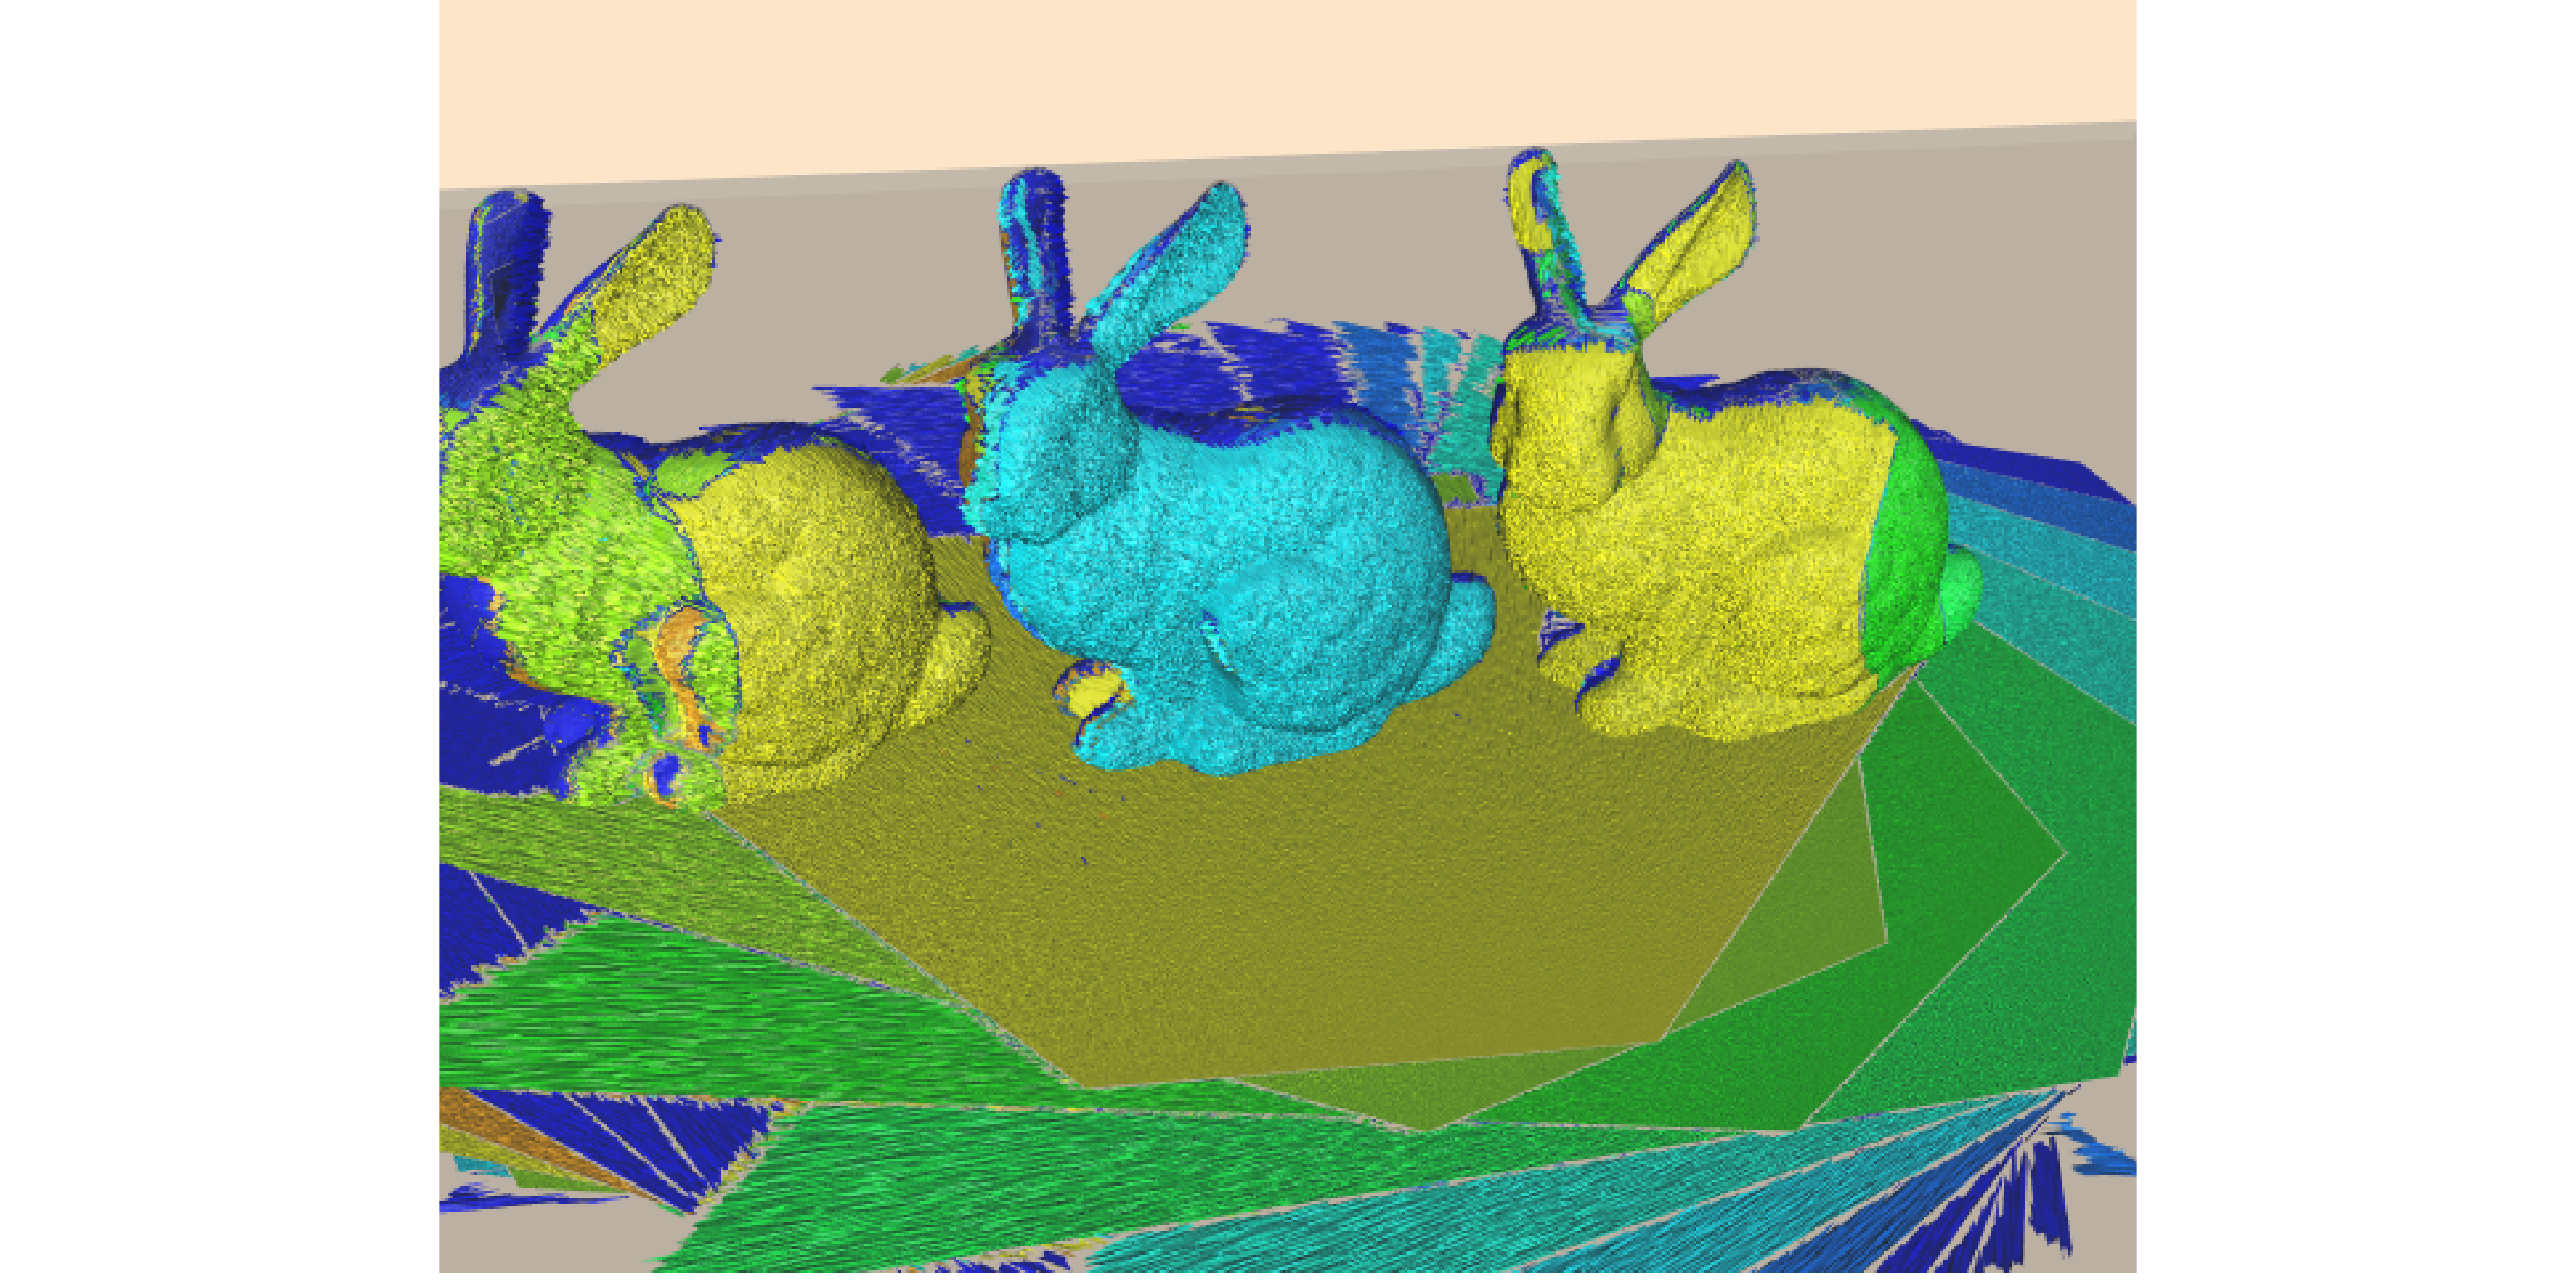
\includegraphics[width=1.2\textwidth]{../figures/results_run3_global_mesh.png}

  \note<1>{\begin{itemize}
    \item Gaps in the mesh
    \item - Traditional methods have overlapping layers
    \item - So you don't notice gaps
    \item The mesh is noisy.
    \item - Our method simply connects
    neighboring points in the point cloud without additional steps such as
    Laplacian smoothing
    \item[]
    \item My reconstruction method was sufficient for demonstrating the
    usefulness of the MABDI algorithm
    \item - mesh has the same magnitude of noise as the sensor's simulated noise
  \end{itemize}}

\end{frame}

\begin{frame}{Mesh Progression} % ______________________________________________
  \vspace{-0.15in}
  \hspace*{-12.5mm}
  \includegraphics[width=1.2\textwidth]<1>{../figures/results_run1_gm.pdf}
  \includegraphics[width=1.2\textwidth]<2>{../figures/results_run2_gm.pdf}
  \includegraphics[width=1.2\textwidth]<3>{../figures/results_run3_gm.pdf}

  \note<1>{\begin{itemize}
    \item[] Traditional methods
    \item would have a plot similar to that indicated by the red arrow on the graph
    \item[] MABDI
    \item levels off as the environment becomes more known
  \end{itemize}}

  \note<2>{\begin{itemize}
    \item MABDI is reactive as the sensor moves to parts of the environment that
    are rich in information
    \item the mesh grows rapidly based on the needs of the environment
  \end{itemize}}

  \note<3>{\begin{itemize}
    \item Large jump in graph corresponding to new bunny
  \end{itemize}}
\end{frame}
